\documentclass[12pt]{article}
\usepackage{times}
\usepackage{graphicx}
\usepackage{amssymb}
\usepackage{xspace}
\usepackage{enumerate}
\usepackage{listings}
\usepackage{url}
\usepackage[usenames,dvipsnames]{xcolor}

\textwidth       6.75in
\textheight      9.25in
\oddsidemargin   -.25in
\evensidemargin  -.25in
\topmargin       -.75in
%\longindentation 0.50\textwidth

\newcommand{\todo}{{\color{green} [Todo]. \xspace}}
\newcommand{\harish}[1]{{\color{blue} Harish: [{#1}]\xspace}}
\newcommand{\nivan}[1]{{\color{green} Nivan: [{#1}]\xspace}}
\newcommand{\hidecomment}[1]{}

\newcommand{\eg}{e.g.,\xspace}
\newcommand{\ie}{i.e.,\xspace}

\pagestyle{empty}

\begin{document}
\lstset{language=C}

\noindent This document explains the process of importing data into the TaxiVis system.
The current version uses a fixed schema represented by the following struct (found in the KdTrip.hpp file):

\begin{lstlisting}
struct Trip {
        uint32_t  pickup_time;
        uint32_t  dropoff_time;
        float     pickup_long;
        float     pickup_lat;
        float     dropoff_long;
        float     dropoff_lat;
        uint32_t  field1;         // extra field to import data
        uint32_t  field2;         // extra field to import data
        uint32_t  field3;         // extra field to import data
        uint32_t  field4;         // extra field to import data
        uint16_t  id_taxi;
        uint16_t  distance;     
        uint16_t  fare_amount;  
        uint16_t  surcharge;    
        uint16_t  mta_tax;      
        uint16_t  tip_amount;   
        uint16_t  tolls_amount; 
        uint8_t   payment_type;
        uint8_t   passengers;       
    };
\end{lstlisting}

\medskip

\noindent This schema includes the attributes present in the data
released by the New York City Taxi \& Limousine Commission (TLC). We have
also included additional attributes (field1, field2, field3 and
field4) to allow for additional data that may be required by different
applications.

\begin{figure}[h]
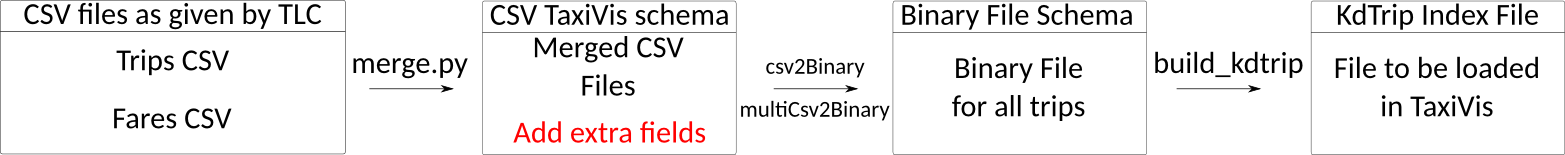
\includegraphics[width=\linewidth]{figs/process.png}
\caption{Summary of the data import process.}
\label{fig:process}
\end{figure}

%\section{Building The Data Index}
\section{Importing the Data and Building the Index}

The source code for building the index is in the src/preprocess
folder. The data import process is illustrated in
Fig.~\ref{fig:process}.
%
The inputs are two separate sets of csv files (provided by the TLC), namely trip and fare files.
%
Two sample data files (sample\_trip\_data\_1.csv and sample\_trip\_fare\_1.csv, one of each type) are included in the \emph{data/rawData} folder.
%
The \emph{merge.py} script is used to merge this files into a single
csv file. This script also adds the placeholder columns \emph{field1,field2,field3,} and \emph{field4} (the default values are all zeros, but additional data might be derived and imported here).
%
It is invoked as follows:
\lstset{language=bash}
\begin{lstlisting}
> python merge.py sample_trip_data_1.csv sample_trip_fare_1.csv merged_test_data.csv
\end{lstlisting}

%
The merged filed is then serialized as a binary file. This is done so
that the index construction can scale to large volumes of data. There
are two programs that can accomplish this job: \emph{csv2Binary} and
\emph{multiCsv2Binary}. 
%Both are really similar, the main difference is
%that 
csv2Binary processes {\bf one} csv file and outputs a
corresponding binary file. It is used as follows:
\lstset{language=bash}
\begin{lstlisting}
./csv2Binary merged_test_data.csv bin_test_data.bin
\end{lstlisting}

multiCsv2Binary has as input a file containing a {\bf list} of csv files to be processed and outputs a single binary file containing all the trips in the input files. An example of input to multiCsv2Binary is the content of the \emph{fileLocations.txt} file shown in the following:
\lstset{language=xml}
\begin{lstlisting}
../../data/rawData/data_1.csv
../../data/rawData/data_2.csv
\end{lstlisting}

The usage multiCsv2Binary is illustrated in the following:
\lstset{language=bash}
\begin{lstlisting}
./multiCsv2Binary fileLocations.txt bin_test_data.bin
\end{lstlisting}

%
Finally, the \emph{build\_kdtrip} script that takes as input the binary file containing the trip records and outputs the kdtrip index that is loaded by TaxiVis. The usage is:
\lstset{language=bash}
\begin{lstlisting}
./build_kdtrip bin_test_data.bin test_data.kdtrip
\end{lstlisting}

\section{Parsing files from TLC website}
TLC now releases the data at \url{http://www.nyc.gov/html/tlc/html/about/trip_record_data.shtml}. To parse this data into TaxiVis format, we can use a process similar to the one described in the previous section. In this new format, fare and trip files are already integrated, so there is no need to use the merge script. Instead we use the parser \emph{newFormatCsv2Binary.cpp} as follows

\lstset{language=bash}
\begin{lstlisting}
././newFormatCsv2Binary yellow_tripdata_2015-01.csv bin_test_data.bin
\end{lstlisting}

Once this is done, we can proceed as before and use the \emph{build\_kdtrip} to build the index to be used in TaxiVis.

\section{Loading File in TaxiVis}
The kdtrip file is loaded by TaxiVis using the constructor of the \emph{QueryManager} class (\emph{querymanager.cpp} file):

\lstset{language=C++}
\begin{lstlisting}
std::string fname = "/path/to/file/test_data.kdtrip";
\end{lstlisting}

Once this change is made and TaxiVis is run, the file will be  loaded.

\section{Configuring how place holder fields are displayed in TaxiVis}
To configure how the placeholder fields are displayed on TaxiVis, we included
a configuration file called \emph{extra\_fields.txt} (located in the data directory).
This is a csv file whose contents have the following format:
\begin{lstlisting}
field1,Screen Name1,Axis Label1,DisplayValue
field2,Screen Name2,Axis Label2,DisplayValue
field3,Screen Name3,Axis Label3,DisplayValue
field4,Screen Name4,Axis Label4,DisplayValue
\end{lstlisting}

The first field represents the internal name used for the attribute in
the code, while the second represents the label shown in the
interface.  The third field contains the text used to label the axis
in the plots that used this field. The last field is a flag
that indicates if this field should be displayed in the interface or
not. It can have two values: 1 (active), and 0 (inactive). 
%In the example above, only fields 1 and 2 are going to be shown in the interface (see Fig.~\ref{fig:interface}).

\begin{figure}[h]
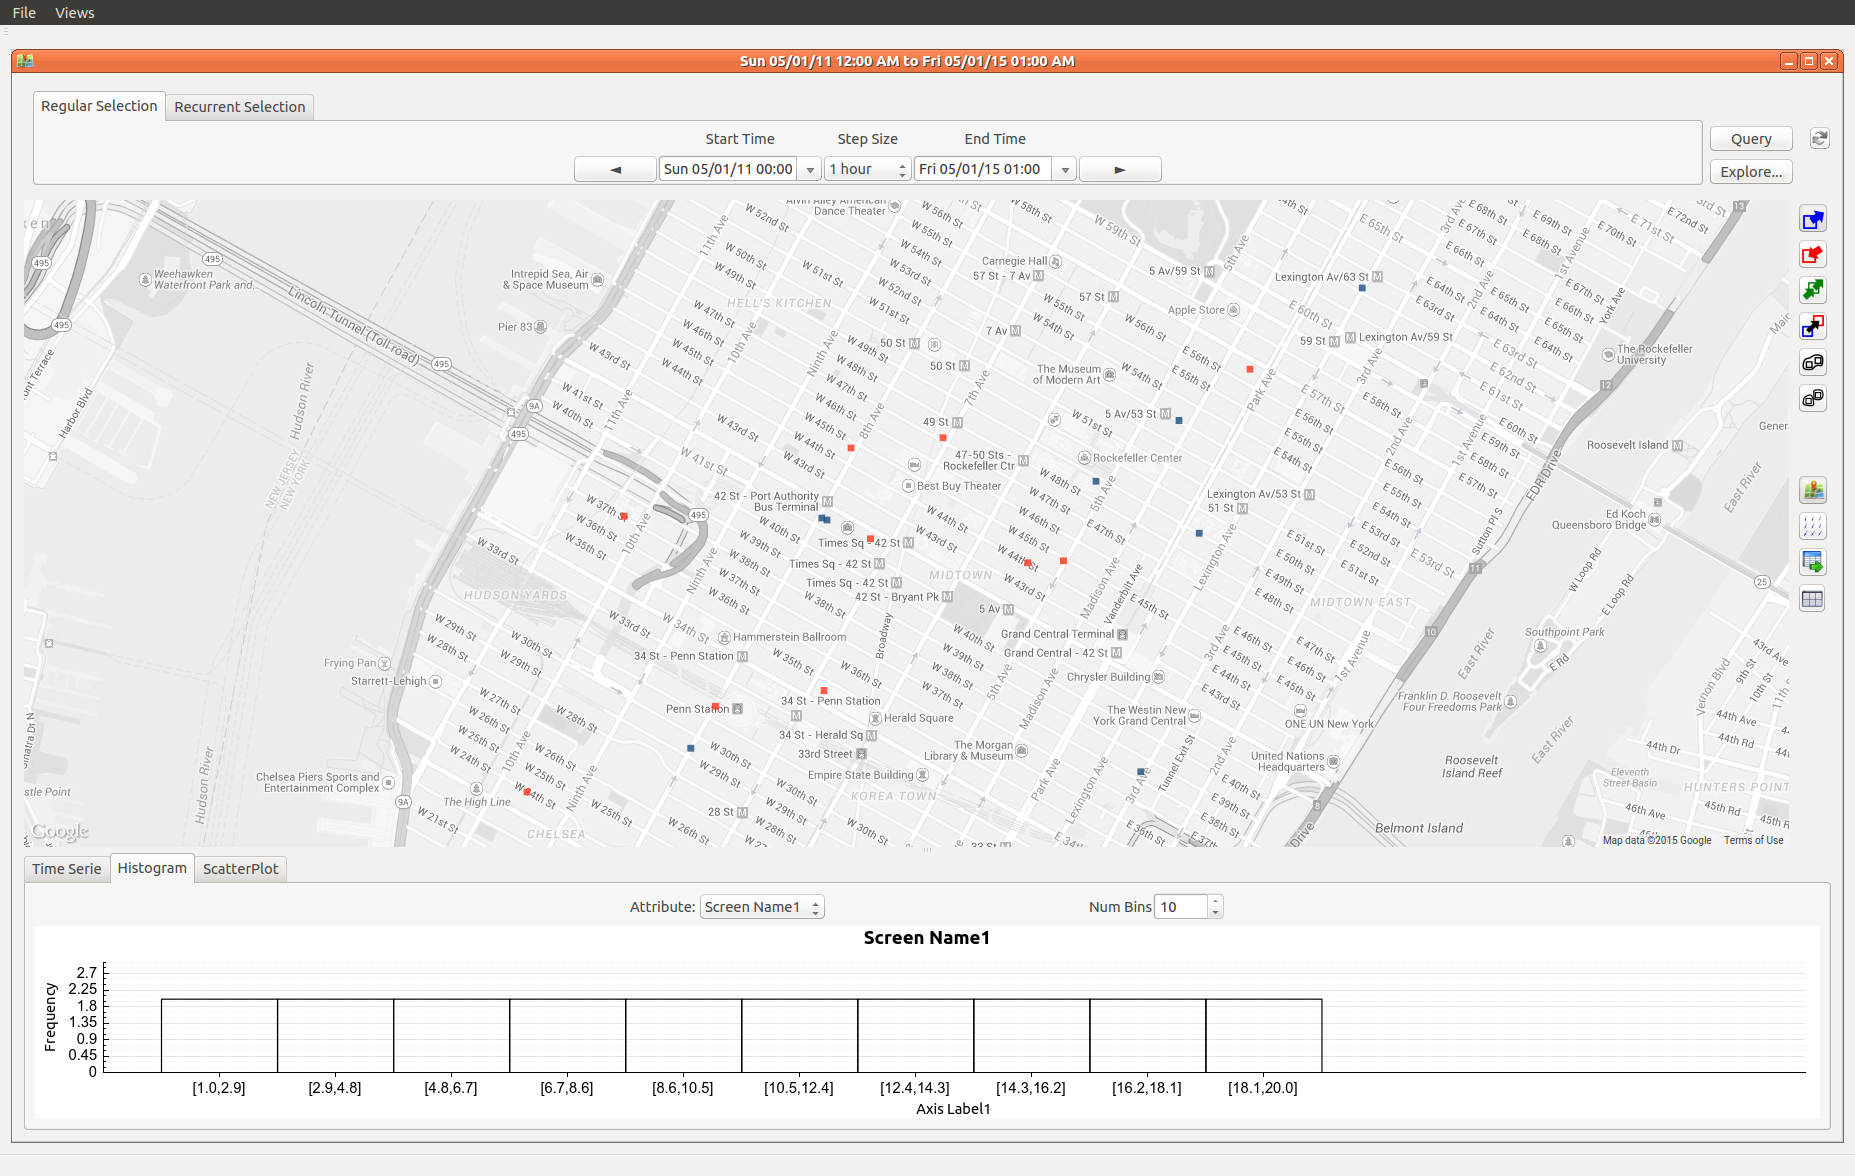
\includegraphics[width=\linewidth]{figs/taxivis.png}
\caption{TaxiVis showing the new data file.}
\label{fig:interface}
\end{figure}


\end{document}
